\newpage
\appendix
\onecolumn

\section{Additional Example Trajectories}
\label{appendix:more_example}
\begin{figure}[h!]
  \centering 
  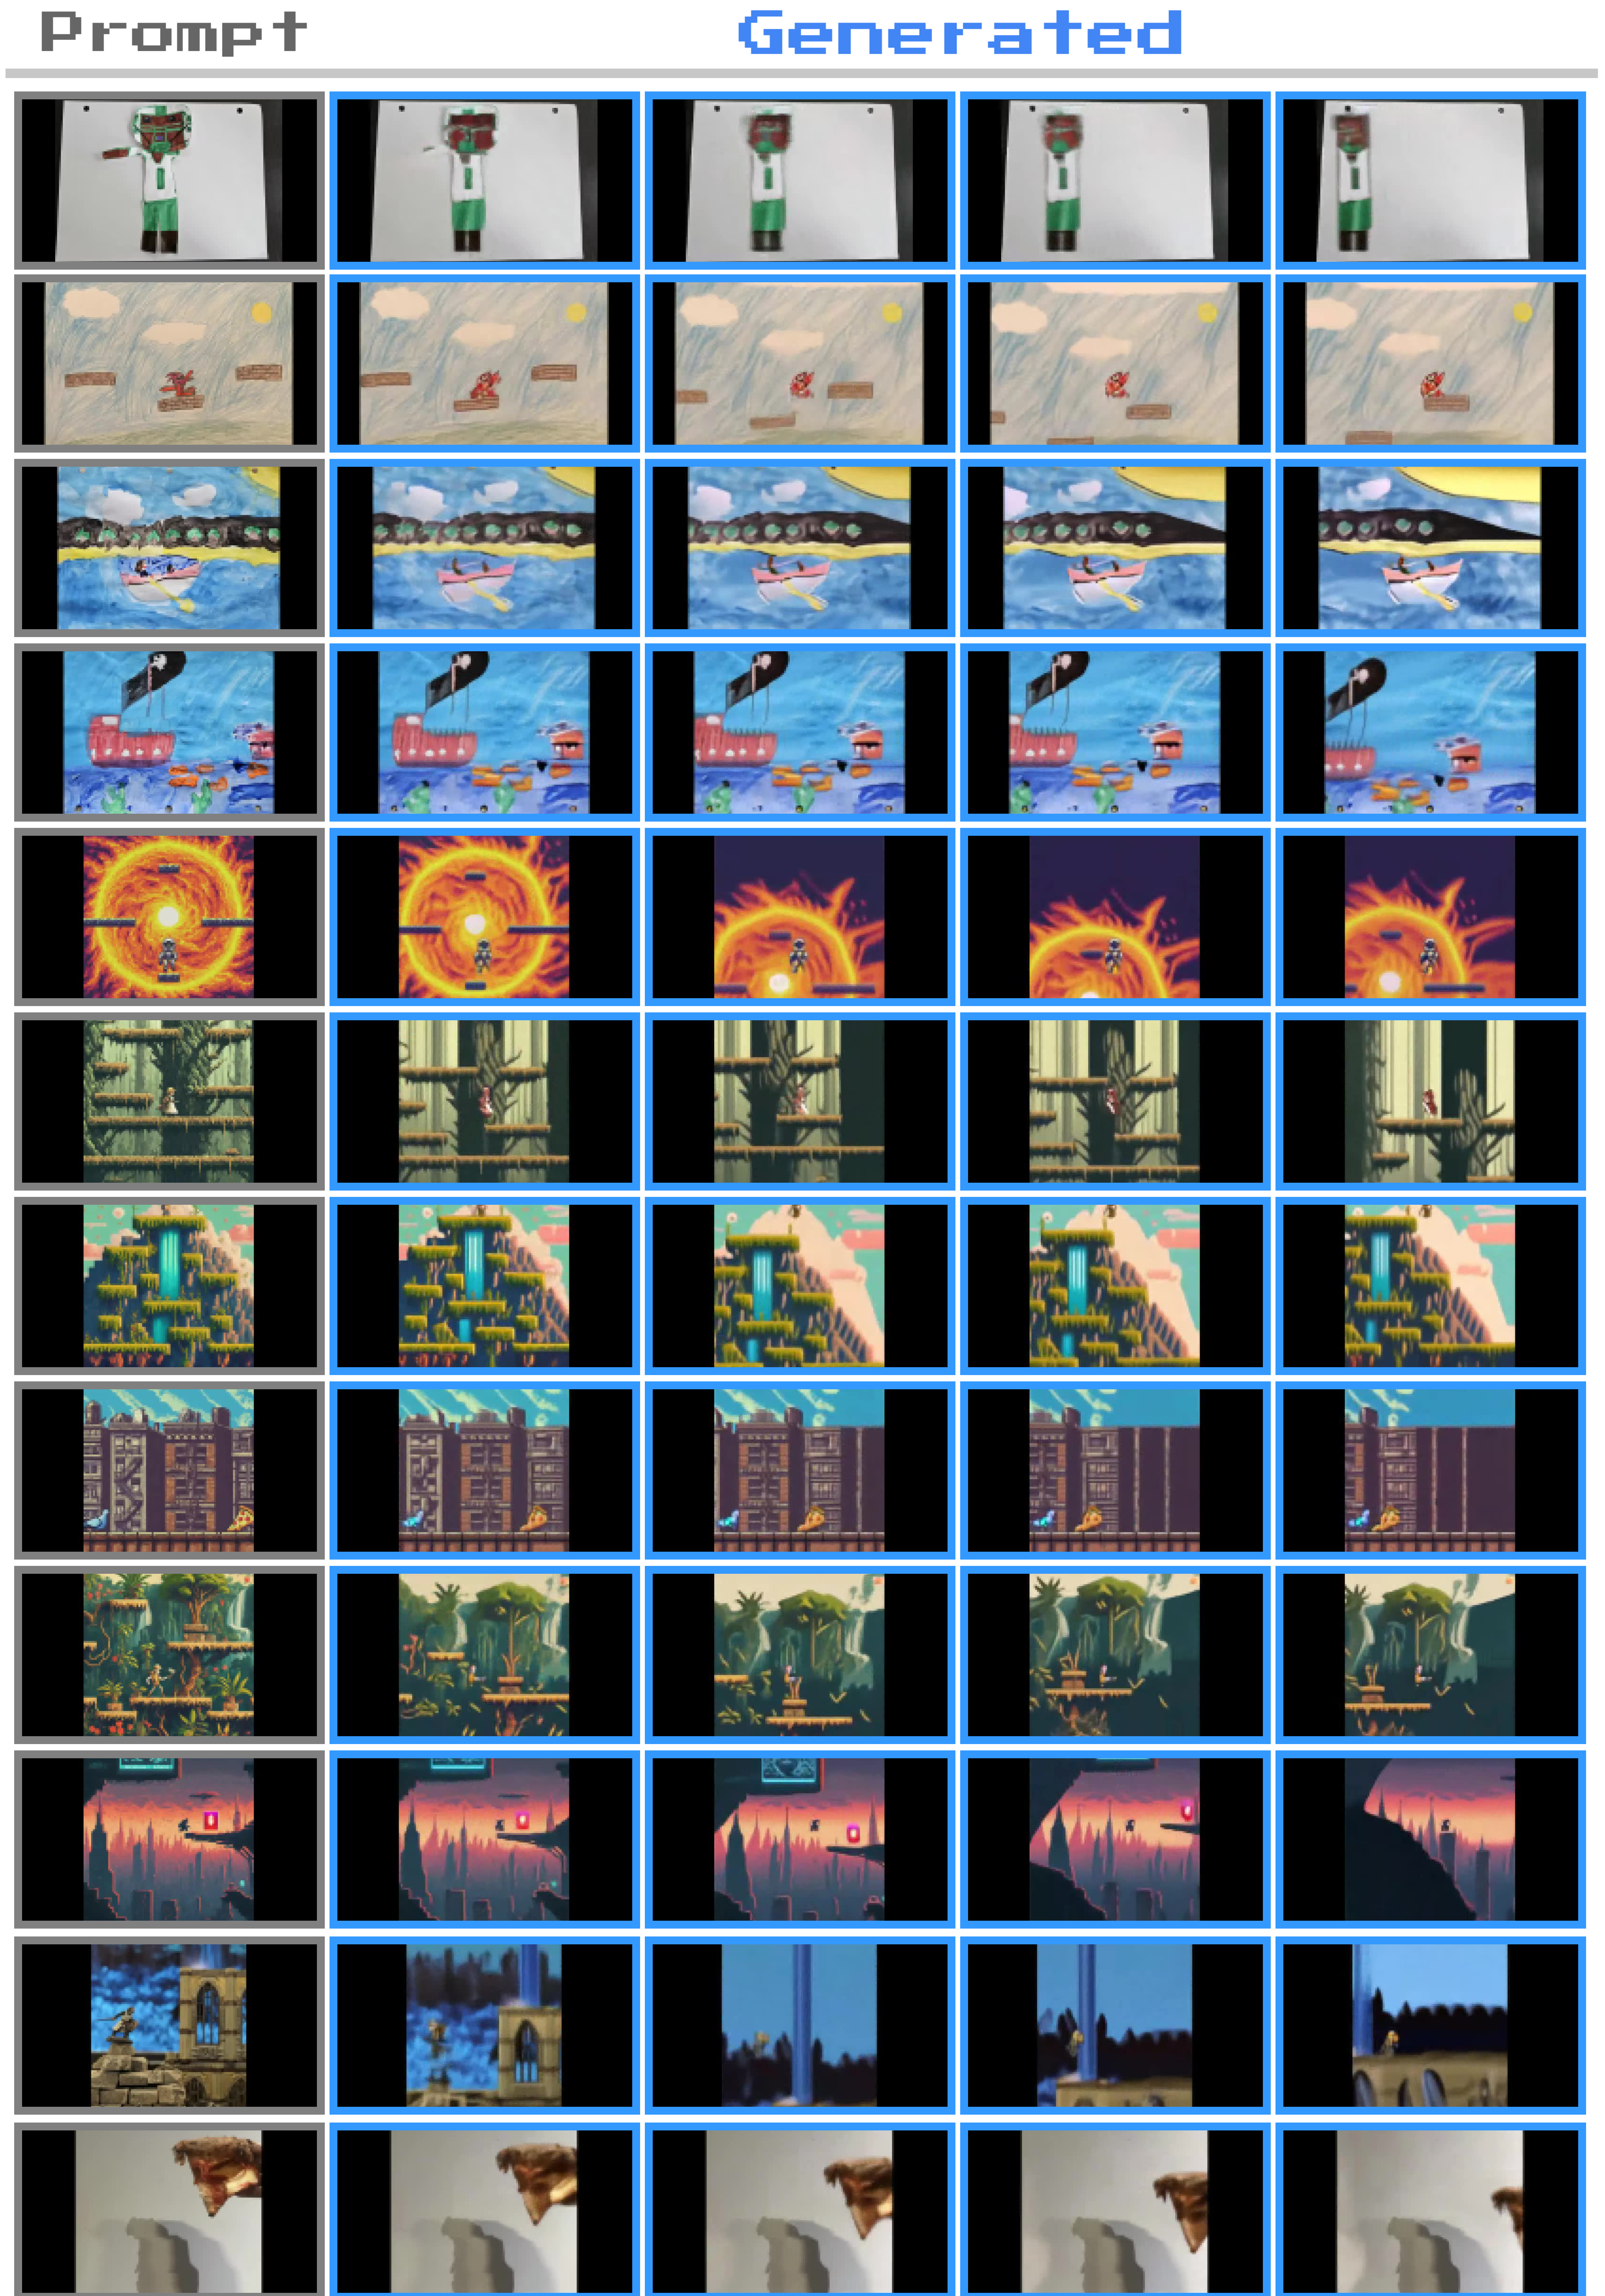
\includegraphics[width=0.85\linewidth]{figures/examples.png}
  \caption{\textbf{More example trajectories}: the model is prompted with either hand-drawn sketches, images generated from text-to-image generative models or realistic photos. Actions that drive the dynamics of the trajectory are provided by human input.}
  \label{fig:more_example}
\end{figure}

\begin{figure}[h!]
    \centering
    \vspace{-2mm}
    \includegraphics[width=0.9\linewidth]{figures/platformers_consistency.pdf}
    \vspace{-1mm}
    \caption{\textbf{Controllable, consistent latent actions in Platformers}: trajectories beginning from four different starting frames from our Platformers dataset. Each column shows the resulting frame from taking the same latent action five times. Despite training without action labels, not only are the same actions consistent across varied prompt frames, but also have semantic meaning: \emph{left}, \emph{right}, \emph{jump}, and \emph{no-op}.}
    \vspace{-3mm}
    \label{fig:consistent_actions_platformers}
\end{figure}


\section{Dataset} \label{sec:app_dataset}

\subsection{Platformers Dataset}
\label{appendix:ytdata}

\paragraph{Initial Dataset} We generated a dataset by filtering publicly available Internet videos, using the following criteria:
\begin{itemize}
    \item The title contains keywords relating to 2D platformer games.
    \item The title or description must contain an action word, such as ``speedrun'' or ``playthrough''.
    \item The title must not contain negating words such as ``movie'' or ``unboxing''.
\end{itemize}
We then split each video into 16s clips at 10 FPS, which corresponds to 160 frames per clip. Our resulting dataset contains 55M videos, which totals around 244k hours. When selecting keywords, we manually spot checked results to check that they typically produced 2D platformer gameplay videos which are not outnumbered by other sorts of videos which happen to share similar keywords.


\paragraph{Filter Pipeline} We noticed that many of the videos in the dataset were of poor quality, impacting our model performance. We propose a scalable approach to systematically filter the data, using a learned classifier as in \cite{baker2022video}. First, we define high quality videos as those that display clear gameplay and do not contain distractor items such as menu screen or streamer faces. We then filter this data as follows:
\begin{enumerate}
    \item Our team hand labelled 10k videos, with roughly ten hours of total human effort. The labels ranged from 5 (best) to 1 (worst) quality.
    \item We trained a 11M parameter ResNet18 \citep{resnet} with binary classification where we deleted all entries rated 2-4 and classified 5 as good and 1 as bad.
    \item We then apply a decision rule based on model prediction and confidence to determine whether to keep the video.
\end{enumerate}
Consistent to findings in prior work \citet{baker2022video, oquab2023dinov2}, having high quality data outweighs the quantity of data -- even though the curated datasaet is only just over 10\% the size of the original dataset, the model trained on the curated dataset outperforms in terms of FVD, see \Cref{tab:dataset_ablation}. Our final dataset is 6.8M videos for a total of over 30k hours.

\begin{table}[h]
\caption{Effect of dataset curation. }
\vspace{3pt}
\label{tab:dataset_ablation}
\centering
\resizebox{.5\textwidth}{!}{
\begin{tabular}{lcc}
\toprule
& \#Params & FVD ($\downarrow$) \\ \midrule
Original dataset (55M videos) & 580M & 61.4 \\ 
Curated dataset (6.8M videos)  & 580M & \textbf{54.8} \\ \bottomrule
\end{tabular}
}
\end{table}

\section{Training details} \label{sec:app_training}
\subsection{Latent Action Model Training}
\label{sec:actionmodel_details}

We found a benefit from increasing the number of codes (i.e. number of actions), at the cost of reduced playability for human and AI agents.

\begin{table}[h]
\caption{Platformers action model hyperparameters}
\label{tab:platformer_actions}
\centering
\small{
\begin{tabular}{llc}
\toprule
Component & Parameter & Value \\ \midrule
Encoder & num\_layers & 20  \\ 
& d\_model  & 1024 \\ 
& num\_heads  & 16 \\ \midrule
Decoder & num\_layers & 20  \\ 
& d\_model  & 1024 \\ 
& num\_heads  & 16 \\ \midrule
Codebook & num\_codes & 8  \\ 
 & patch\_size & 16  \\ 
& latent\_dim  & 32 \\ \bottomrule
\end{tabular}}
\end{table}

Note that the model inputs are normalized between $0$ and $1$ and the final outputs of the decoder are placed through a sigmoid. 

\subsection{Video Tokenizer Training}
\label{sec:vidtok_details}

Here we describe our video tokenizer training. We found it more effective to scale our decoder than the encoder, and a marginal gain from increasing batch size (see Table~\ref{tab:batch_size_hps_tokenizer}).

\begin{table}[h]
\centering
\caption{Tokenizer batch size scaling hyperparameters.}
\label{tab:batch_size_hps_tokenizer}
\resizebox{.5\textwidth}{!}{
\begin{tabular}{lccc}
\toprule
batch\_size & training hardware & FLOPs & PSNR \\ \midrule
64 & 64 TPUv2 & $4.22 \times 10^{20} $ & 35.7 \\ 
384 & 64 TPUv3 & $2.57 \times 10^{21} $ & 36.5 \\ 
\bottomrule
\end{tabular}
}
\end{table}


\begin{table}[h]
\caption{Platformers video tokenizer hyperparameters.}
\label{tab:platformers_vid_tok}
\centering
\small{
\begin{tabular}{llc}
\toprule
Component & Parameter & Value \\ \midrule
Encoder & num\_layers & 12  \\ 
& d\_model  & 512 \\ 
& num\_heads  & 8 \\ 
& k/q\_size  & 64 \\ \midrule
Decoder & num\_layers & 20  \\ 
& d\_model  & 1024 \\ 
& num\_heads  & 16 \\
& k/q\_size  & 64 \\ \midrule
Codebook & num\_codes & 1024  \\ 
  & patch\_size & 4  \\ 
& latent\_dim  & 32 \\ \bottomrule
\end{tabular}}
\end{table}

We train our video tokenizer for 300k steps using the AdamW optimizer, with cosine decay, using the hyperparameters in Table~\ref{tab:vid_tok_adam}.

\begin{table}[h]
\caption{Video tokenizer optimizer hyperparameters}
\label{tab:vid_tok_adam}
\centering
\small{
\begin{tabular}{lc}
\toprule
Parameter & Value \\ \midrule
max\_lr & 3e-4  \\ 
min\_lr  & 3e-4 \\ 
$\beta_1$  & 0.9 \\ 
$\beta_2$  & 0.9 \\ 
weight\_decay & 1e-4 \\ 
warmup\_steps & 10k \\ \bottomrule
\end{tabular}}
\end{table}

\subsection{Dynamics Model Training}
\label{sec:dynamicsmodel_details}

\begin{table}[h]
\caption{Dynamics model optimizer hyperparameters}
\label{tab:dynamics_model_adam}
\centering
\small{
\begin{tabular}{lc}
\toprule
Parameter & Value \\ \midrule
max\_lr & 3e-5  \\ 
min\_lr  & 3e-6 \\ 
$\beta_1$  & 0.9 \\ 
$\beta_2$  & 0.9 \\ 
weight\_decay & 1e-4 \\ 
warmup\_steps & 5k \\ \bottomrule
\end{tabular}}
\end{table}

\section{Scaling Experiments Details} \label{sec:app_scaling_details}

In this section we provide more details on the architecture as well as compute budget for the scaling experiments. 

\paragraph{Scaling model size} For all models we use a batch size of 256. We train all models for 200k steps, thus use a total of 750B training tokens for each run. All runs make use of batch parallelism and stage-3 ZeRO sharding \citep{rajbhandari2020zero}, while our larger models also make use of tensor parallelism \citep{megatron}. For this experiment we make use of TPUv2 and TPUv3 \citep{jouppi2020domain}. See Table~\ref{tab:model_size_hps} for more details.


\begin{table}[h]
\centering
\caption{Model size scaling architectures and compute usage. All models were trained for 200k steps with a batch size of 256, equating to 750B tokens.}
\label{tab:model_size_hps}
\resizebox{.85\textwidth}{!}{
\begin{tabular}{lccccccc}
\toprule
Parameters & num\_layers & num\_heads & d\_model & k/q size & training hardware & training time & FLOPs \\ \midrule
41M & 18 & 8 & 512 & 64 & 64 TPUv2 & 3 days & $2.05 \times 10^{20}$ \\ 
96M & 16 & 16 & 768 & 64 & 64 TPUv2 & 6 days & $3.58 \times 10^{20}$ \\ 
192M & 20 & 18 & 1024 & 64 & 64 TPUv2 & 9 days & $6.4 \times 10^{20}$ \\ 
404M & 21 & 12 & 1536 & 128 & 64 TPUv2 & 18 days & $1.2 \times 10^{21}$ \\
811M & 20 & 20 & 2048 & 128 & 128 TPUv3 & 7 days & $2.2 \times 10^{21}$ \\
1.6B & 28 & 22 & 2560 & 128 & 128 TPUv3 & 12 days & $4.04 \times 10^{21}$ \\
2.7B & 36 & 22 & 3072 & 128 & 256 TPUv3 & 16 days & $6.91 \times 10^{21}$ \\ 
\bottomrule
\end{tabular}
}
\end{table}

\paragraph{Scaling batch size}  All models use the same architecture with 2.3B parameters, as shown in Table~\ref{tab:batch_size_hps}, and train for 200k steps. The only difference between the three runs is hardware---the 128, 256 and 448 batch size models train on 64 TPUv3, 128 TPUv3 and 64 TPUv5p respectively.  

\begin{table}[h]
\centering
\caption{Batch size scaling hyperparameters. All models use the following architecture for 200k steps, differing only in batch size.}
\label{tab:batch_size_hps}
\resizebox{.5\textwidth}{!}{
\begin{tabular}{lcccc}
\toprule
Parameters & num\_layers & num\_heads & d\_model & k/q size \\ \midrule
2.3B & 34 & 20 & 2560 & 128 \\ 
\bottomrule
\end{tabular}
}
\end{table}


\paragraph{Genie Model} The parameter count, model architecture as well as compute usage of the dynamics model for the final Genie model is listed in \Cref{tab:genie_11b}. We train a 10.1B dynamics model with a batch size of 512, for a total of 125k steps using 256 TPUv5. 
\begin{table}[h]
\centering
\caption{Genie dynamics model hyperparameters.}
\label{tab:genie_11b}
\resizebox{.55\textwidth}{!}{
\begin{tabular}{lccccc}
\toprule
Parameters & num\_layers & num\_heads & d\_model & k/q size & FLOPs \\ \midrule
10.1B & 48 & 36 & 5120 & 128 & $6.6\times 10^{22}$ \\ 
\bottomrule
\end{tabular}
}
\end{table}

\section{Behavioral Cloning Details}
\label{appendix:bc}
In this section we provide more details about our behavioral cloning experiments. We train within the Procgen CoinRun environment~\citep{procgen} and evaluate in a held out test set. We assume we have a dataset of expert sequences in this environment from an agent trained with R2D2~\citep{kapturowski2018recurrent}. We then train an agent to imitate from this data. Notably, the oracle agent has access to the corresponding ground-truth expert actions. We now discuss how we can utilize a pre-trained LAM to infer the actions taken.

\subsection{Genie LAM}
In order to train an agent to imitate from unseen videos, we can use a frozen LAM from a Genie model trained on Internet videos. Given an expert sequence $\langle x_t, x_{t+1} \rangle$ we extract the corresponding latent action label $a_{t} \leftarrow LAM(x_t, x_{t+1})$. We then train a policy $\pi(a_t|x_t)$ to predict the likelihood of the expert taking latent action $a_t$ given observation $x_t$. Note that this procedure is similar to prior works that learn from videos \citep{torabi2018behavioral, baker2022video}. However, these approaches use ground-truth actions for labeling videos whereas we utilize latent actions learnt completely offline.

During inference, we must map latent actions emitted by the policy to real actions. To do this, we utilize a small set of action-labeled expert sequences. Given an expert sequence $\langle x_t, u_t, x_{t+1} \rangle$ (we denote $u_t$ for ground-truth actions to avoid confusion with predicted latent actions), we use the LAM to obtain a latent action $a_t$ and fill a dictionary $D$ consisting of mapped latents to a list of corresponding real actions. In summary, given an observation $x_t$ from the environment, we can obtain the most likely latent action as $a_t \sim \pi(s_t)$, and then take the corresponding real action as $u_t \sim D[a_t]$.

Note that other works have used data extracted from the agent's policy to obtain a mapping from latent to real actions \citep{edwards2019imitating, ye2022become}, but we found using expert data enabled us to better evaluate the quality of the learnt policy. As shown in the main text, the agent was capable of adapting with as few as $200$ expert labels. 

\subsection{Architecture}
We train a transformer as the policy for both the oracle and latent BC agents. We utilize our proposed ST-ViViT architecture for encoding the frames $\x_{1:t}=(x_1,\cdots x_t)$ . All previous actions are placed through a one-hot and then combined with the corresponding frame encoding as an additive embedding. We use a sequence length of $4$ during both training and inference and a batch size of $16$. 

\begin{table}[h!]
\caption{BC model optimizer hyperparameters}
\label{tab:bc_model_adam}
\centering
\small{
\begin{tabular}{lc}
\toprule
Parameter & Value \\ \midrule
max\_lr & 3e-5  \\ 
min\_lr  & 3e-6 \\ 
$\beta_1$  & 0.9 \\ 
$\beta_2$  & 0.96 \\ 
weight\_decay & 1e-4 \\ 
warmup\_steps & 5k \\ \bottomrule
\end{tabular}}
\end{table}

\begin{table}[h!]
\caption{BC policy hyperparameters}
\label{tab:bc_actions}
\centering
\small{
\begin{tabular}{llc}
\toprule
Component & Parameter & Value \\ \midrule
Encoder & num\_layers & 12  \\ 
& d\_model  & 512 \\ 
& patch\_size  & 4 \\ \midrule
Policy & linear\_layer & 512  \\ \bottomrule
\end{tabular}}
\end{table}

Both the oracle and Genie LAM are trained with a cross-entropy loss where targets are either real or latent actions, respectively. During inference, we obtain the final prediction by sampling from the predicted logits. Note we found the oracle agent performed better when we randomly sampled actions $10\%$ of the time. 


\section{Reproducible Case Study} \label{appendix:case_study}

In this section we describe a self-contained, fully reproducible case study that can be trained with a single mid range TPU/GPU in under a week. 

\subsection{Data Collection}

First we need to collect the data to train our model. We use the CoinRun environment from the Procgen benchmark \citep{procgen} since it has thousands of visually diverse levels with fairly simple platformer-like dynamics. Using the ``hard'' mode, we collect data using a random policy with no action repeats. We sample level seeds between zero and 10,000 and collect 1,000 timesteps for each level, for a total of 10M transitions.

\subsection{Video Tokenizer Training}
 
Our video tokenizer for CoinRun follows the same setup as described in Section~\ref{sec:model_components}, trained with the optimizer configuration as in Section~\ref{sec:vidtok_details}. The primary difference in this example is we use smaller model sizes (see Table~\ref{tab:coinrun_vid_tok}), and then use a batch size of 48 sequences, of length 16, for a total of 768 images per batch. This is sufficient to fit in a single TPU with 16G memory. The model is trained for three days using a single TPU which is sufficient to complete 300k steps.  

\begin{table}[h]
\caption{CoinRun video tokenizer hyperparameters}
\label{tab:coinrun_vid_tok}
\centering
\small{
\begin{tabular}{llc}
\toprule
Component & Parameter & Value \\ \midrule
Encoder & num\_layers & 8  \\ 
& d\_model  & 512 \\ 
& num\_heads  & 8 \\ \midrule
Decoder & num\_layers & 8  \\ 
& d\_model  & 512 \\ 
& num\_heads  & 8 \\ \midrule
Codebook & num\_codes & 1024  \\ 
  & patch\_size & 4  \\ 
& latent\_dim  & 32 \\ \bottomrule
\end{tabular}}
\end{table}

\subsection{Dynamics + Latent Action Model Training}

Once we have trained the video tokenizer we can then jointly train the latent action and dynamics models. Once again we seek to fit our model training inside 16G memory, so we use a batch size of 36 sequences consisting of 16 frames each, for a total of 576 images. We train both the latent action model and dynamics model in parallel, using the setup described above (see: Section~\ref{sec:actionmodel_details} for the latent action model and Section~\ref{sec:dynamicsmodel_details} for the dynamics model).

We train both the latent action and dynamics models in parallel for 200k steps, using the optimizer hyperparameters in \Cref{tab:dynamics_model_adam}. We find this model generates consistent playable latent actions, resembling the original environment.

\begin{table}[h]
\caption{CoinRun action model hyperparameters}
\label{tab:coinrun_actions}
\centering
\small{
\begin{tabular}{llc}
\toprule
Component & Parameter & Value \\ \midrule
Encoder & num\_layers & 8  \\ 
& d\_model  & 512 \\ 
& num\_heads  & 8 \\ \midrule
Decoder & num\_layers & 8  \\ 
& d\_model  & 512 \\ 
& num\_heads  & 8 \\ \midrule
Codebook & num\_codes & 6  \\ 
& latent\_dim  & 32 \\ \bottomrule
\end{tabular}}
\end{table}

\begin{table}[h]
\caption{CoinRun dynamics model hyperparameters}
\label{tab:coinrun_dynamics}
\centering
\small{
\begin{tabular}{lcc}
\toprule
Component & Parameter & Value \\ \midrule
Architecture & num\_layers & 12  \\ 
& d\_model  & 512 \\ 
& num\_layers  & 8 \\ 
Sampling & temperature  & 1.0 \\ 
& maskgit\_steps  & 25 \\ \bottomrule
\end{tabular}}
\end{table}
